\documentclass[11pt]{article}
\usepackage[margin=1in]{geometry}
\usepackage{fontspec}
\usepackage{xeCJK}
\setmainfont{Times New Roman}
\setCJKmainfont[AutoFakeBold=2.5,AutoFakeSlant=.2]{SimSun}
\setCJKsansfont{SimHei}
\setCJKmonofont{SimSun}
\usepackage{amsmath,amssymb,amsthm}
\usepackage{booktabs,longtable,array}
\usepackage{tikz}
\usetikzlibrary{arrows.meta,positioning}
\usepackage{hyperref}
\hypersetup{colorlinks=true,linkcolor=blue,citecolor=blue,urlcolor=blue,pdftitle={无限自由五子棋先手必胜的计算机辅助证明（中文译本）},pdfauthor={Gaoqiang Liu}}
\usepackage{microtype}
\linespread{1.10}
\renewcommand{\abstractname}{摘要}
\renewcommand{\figurename}{图}
\renewcommand{\tablename}{表}
\renewcommand{\refname}{参考文献}
\renewcommand{\proofname}{证明}
\newtheorem{theorem}{定理}[section]
\newtheorem{lemma}[theorem]{引理}
\newtheorem{proposition}[theorem]{命题}
\newtheorem{corollary}[theorem]{推论}
\theoremstyle{definition}
\newtheorem{definition}[theorem]{定义}
\theoremstyle{remark}
\newtheorem{remark}[theorem]{说明}
\newcommand{\Z}{\mathbb Z}
\newcommand{\N}{\mathbb N}
\newcommand{\dist}{\lVert\,\cdot\,\rVert_\infty}
\newcommand{\A}{\alpha}
\newcommand{\Win}{\operatorname{Win}}
\newcommand{\Succ}{\operatorname{Succ}}
\newcommand{\code}[1]{\texttt{#1}}
\title{无限自由五子棋先手必胜的计算机辅助证明\\\large 中文阅读译本}
\author{Gaoqiang Liu\thanks{依独立审阅意见修订的阅读稿，尚未经过外部同行评审。完整证书的可移植交付状态见第~\ref{sec:repro} 节。}\\拜罗伊特大学，德国拜罗伊特\\\href{mailto:Gaoqiang.Liu@uni-bayreuth.de}{\texttt{Gaoqiang.Liu@uni-bayreuth.de}}}
\date{2026年10月4日}
\begin{document}
\maketitle

\begin{abstract}
我们给出一个计算机辅助证明：在无限整数格点上的自由式五子棋中，先手获胜。
双方轮流占据一个空格点；在四个方向中的任一方向形成至少五子的连续连线，
便立即获胜；双方均无禁手。经认证的策略从原点落子开始，能在双方合计
不超过 35 次落子内先于后手获胜。有限证明对象采用一种保守抽象，
在两个坐标轴上分别将相邻坐标间距截断至五。我们证明了获胜连线的保持性、
对后手每一个合法落子的覆盖性，以及相对先手着法在每个实际原像中的可实施性。
因此，远处的落子得到表示，而非被视为无害的停着。
利用对称性，后手的第一次回应被约化为 20 个轨道，覆盖 120 个规范化局面。
有界威胁规则压缩了策略的部分内容，同时保留反威胁和实际落子次数。
独立于搜索的检查器重建后继集合，并检查完整的依赖闭包。
我们说明数学上的可靠性论证、已记录的验证过程以及可移植发布的要求。
这个界是上界，并不声称其为最优。
\end{abstract}

\section{引言}
\label{sec:intro}
五子棋是一种强位置博弈：双方都能通过完成规定的连线获胜，
而双方完成各自连线的先后次序至关重要。本文研究的是无限棋盘，
而非有限棋盘边界规则的扩展。双方都可以使用 $\Z^2$ 的每一个点。
特别是，后手可以在先手开始进攻的区域之外构筑威胁，迫使先手防守，
并在之后连接先前彼此分离的棋子。证明必须涵盖所有这些可能性，
以及后手先获胜的情况。

有限棋盘上的结果是一个重要的计算先例。Allis、van den Herik 和 Huntjens
解决了 $15\times15$ 棋盘上的两种无禁手变体，包括长连获胜的变体
\cite{Allis1993,Allis1996}。他们的威胁空间搜索和证明数搜索
也为生成候选策略提供了思路。不过，有限棋盘上的策略本身
并不是无限棋盘上的策略。额外的格点不仅为后手增加了合法回应，
也增加了获胜连线。边界可能有助于先手履行防守义务；
在强博弈中，移除边界并不是一种单调变化。

我们的贡献是针对无限棋盘自由式规则给出一个有限且可独立检查的证明对象。
其核心数学工具是动态坐标间距抽象。它保留双方的每一颗棋子，
精确记录所有较小的坐标差，并对较大间距采用有限的保守转移集合。
先手着法相对于一颗已有棋子指定，并针对每一种可能的抽象结果进行检查。
因此，这个策略在证书节点所表示的每一个实际格点局面上都有相应解释。
抽象可以包含额外结果，但必须覆盖所有实际结果，并为每个列出的结果提供经认证的后续策略。

主要结果如下。
\begin{theorem}[无限棋盘自由式五子棋]
\label{thm:main}
在 $\Z^2$ 上，黑棋先行，双方交替在空点落子，无禁手；
在水平、垂直或两个对角方向之一形成至少五子的连续连线便立即获胜。
在这些规则下，黑棋具有一个首着为 $(0,0)$ 的策略，
对每一个合法的白棋策略，都能先于白棋获胜。
从空棋盘开始计数，获胜发生在双方合计至多 35 次实际落子之后。
\end{theorem}

证明分为两部分。数学部分证明：获接受的证书规则蕴含实际无限棋盘上的策略。
计算部分验证一个满足这些规则的具体有限证书。
检查器不信任引擎估值、搜索成功标签或被省略的分支。
结论既不声称 35 是可能的最小统一上界，也不声称每一盘都持续 35 步。


\subsection{相关工作与结论的范围}
文献回顾区分了双方均可能先获胜的强博弈，以及后手仅负责阻止先手的
弱 Maker--Breaker 博弈。弱博弈的结果不会自动解决强博弈。
Erde 关于有偏 $n$ 子连线博弈的工作也使用了不同的行棋协议
\cite{Erde2012}。针对更大目标的配对策略 \cite{Gyorffy2019}
研究的是防守策略，并采用了不同的目标连线长度。
发表于 2014、2019 和 2022 年的综述与论述将无限棋盘强五子连线问题
描述为尚未解决 \cite{Hefetz2014,Gyorffy2019,Pluhar2022}。
这些引用记录了相应日期的文献判断。

另一个逻辑区别涉及有界对局。在一般的无限分支博弈中，
即使每一盘具体对局都会终止，获胜策略也未必具有统一的有限获胜时间上界。
Hamkins 和 Leonessi 讨论的局部性结果在处理简单落子博弈时明确排除了五子棋
\cite{Hamkins2023}。我们的统一上界来自证书中的实际秩和有界策略，
而非关于任意五子棋策略的紧致性断言。

特别是，从强博弈转移到弱博弈，会移除阻止对手完成自身连线的义务。
它并不能证明反向转移是合理的。因此，有限 $15\times15$ 棋盘上的解法
提供了无限棋盘弱博弈的先例，而本文的强博弈证明必须增加对白棋先获胜的检查。
Allis 及合作者描述了 35 半步主变化，并在表 5 中报告两种有限棋盘变体的解答树深度均为 35 \cite{Allis1993}。其树采用威胁空间压缩和白着约减，并处理防守方反冲四。这些有限棋盘统计不能确立无限棋盘上界。本文的 35 计入双方每次实际落子，包括反冲四中断和最终获胜的一手，并覆盖所有无限棋盘防守。

\section{规则与有限局面}
\label{sec:rules}
令
\[
 D=\{(1,0),(0,1),(1,1),(1,-1)\}.
\]
五连段是形如 $L=\{s+id:0\leq i\leq4\}$ 的集合，其中 $s\in\Z^2$
且 $d\in D$。有限局面是由黑棋与白棋所占据的点构成的两个有限且不交的
集合组成的有序对 $P=(B,W)$。记 $|P|=|B|+|W|=p$，表示
其实际落子次数。可达的非终局局面或者满足 $|B|=|W|$，轮到黑棋行棋，
或者满足 $|B|=|W|+1$，轮到白棋行棋。
若某一颜色的棋子集合包含一个五连段，该颜色便已获胜。
这个定义涵盖所有更长的连续连线，因为每一条都包含一个五连段。
每盘对局均在首次出现获胜落子时结束。

设 $S,T\subseteq\Z^2$ 为有限且不交的占据点集，分别表示当前考察的一方与对方。若 $S$ 不含五连段，定义
\[
 \Win(S,T)=\{q\in\Z^2\setminus(S\cup T):
              S\cup\{q\}\text{ 含有一个五连段}\}.
\]
这是立即获胜的落子点集合。在上述未获胜的假设下，对于有限的 $S$，
这个集合是有限的：每一个这样的落子都与四颗原有棋子组成一个五连段。
此记号也用于威胁规则引入的虚拟有限局面；虚拟棋子总会被明确标识，
并不改变实际落子次数 $p$。这些用法满足同样的未获胜假设。
已获胜的集合属于终局，直接接受检测，而不传入这个定义。

证书语言对黑棋着法的限制，是对所认证策略的限制，而非对博弈的限制。
规则上，黑棋可以在任意空点落子。只需使用较小的着法语言认证一个获胜策略即可。
白棋不受类似的搜索限制：必须覆盖白棋的每一个合法落子点。

\section{动态坐标间距}
\label{sec:gaps}
\subsection{规范化与实际原像}
对于任一坐标轴，将 $B\cup W$ 中所有点的互异坐标值，
连同固定锚点 $0$，按顺序排列：
\[
 v_0< v_1<\cdots<v_m.
\]
若 $v_j=0$，在这些值上定义一个严格递增映射 $f$，满足
\[
 f(v_j)=0,\qquad f(v_{i+1})-f(v_i)=\min(v_{i+1}-v_i,5).
\]
独立应用两个映射，得到规范化
\[
 \A(P)=\bigl(\{(f_x(x),f_y(y)):(x,y)\in B\},
             \{(f_x(x),f_y(y)):(x,y)\in W\}\bigr).
\]
锚点是一种坐标约定，并非额外棋子。规范化保留颜色、棋子身份、占据情况、
行棋方以及实际落子次数。规范化局面 $Q$ 表示每一个局面 $P$，只要 $\A(P)=Q$。
等于五的规范化相邻间距，表示任意长度至少为五的实际相邻间距。
因此，一个抽象局面通常具有无穷多个实际原像。

\begin{lemma}[较小坐标差的精确性]
\label{lem:short}
对任意两个已有坐标值 $u,v$，若 $|u-v|\leq4$，则
$f(v)-f(u)=v-u$。反之，若 $|f(v)-f(u)|\leq4$，同样的等式
成立。若 $|u-v|>4$，则 $|f(v)-f(u)|>4$。
\end{lemma}
\begin{proof}
设 $u<v$，并将它们之间的相邻间距相加。若其总和至多为四，
则每个间距都小于五，因而均不发生变化。若出现一个长度至少为五的间距，
则仅其规范化长度就等于五，因此规范化后的总和大于四。
若不存在这样的间距，总和保持不变。这证明了所有断言；
反向排列的情形由改变符号得到。
\end{proof}

\begin{lemma}[获胜连线与占据情况的保持性]
\label{lem:five}
规范化在已有点上是单射，并且在两个方向上都保持任一颜色的五连段的存在性。
\end{lemma}
\begin{proof}
每个坐标轴映射都严格递增，因此两个不同的已有点仍然不同。
在五连段中，任意一对点在每个坐标轴上的差的绝对值都至多为四。
引理~\ref{lem:short} 保持这些有符号差，包括零差。
因此，其像是具有相同方向的五连段。反之，任何构成规范化五连段的五个点之间，
其有符号差的绝对值都至多为四，所以它们的实际差恰好等于该线段中的差。
同样的论证分别适用于每一种颜色。长度大于五的连线包含一个五连段，
因此长连无须特别例外。
\end{proof}

\begin{figure}[ht]
\centering
\begin{tikzpicture}[x=0.58cm,y=0.75cm,>=Stealth]
\draw[->] (-0.5,2)--(13,2);
\foreach \x/\lab in {0/0,2/2,10/40,12/42}
 {\fill (\x,2) circle (2pt);\node[above] at (\x,2) {$\lab$};}
\node[below] at (1,2) {2};\node[below] at (6,2) {38};\node[below] at (11,2) {2};
\draw[->] (-0.5,0)--(13,0);
\foreach \x/\lab in {0/0,2/2,7/7,9/9}
 {\fill (\x,0) circle (2pt);\node[below] at (\x,0) {$\lab$};}
\node[above] at (1,0) {2};\node[above] at (4.5,0) {5};\node[above] at (8,0) {2};
\draw[->,thick] (6,1.1)--(6,0.7);
\node[right] at (6,0.9) {$g\mapsto\min(g,5)$};
\node[left] at (-0.5,2) {实际};\node[left] at (-0.5,0) {规范化};
\end{tikzpicture}
\caption{单轴规范化。上图是示意图，未按比例绘制。
较小间距保持精确；长度为 38 的间距变为长度为五的饱和间距。
该操作应用于双方棋子与锚点的坐标值，而不只是进攻方的棋子。}
\label{fig:gap}
\end{figure}

\subsection{白棋的所有落子都有有限代表}
假设已有坐标值已规范化。插入的坐标或者等于某个已有值，
或者位于两个极端值之外，或者分割某个已有相邻间距。
保留等值插入，因为具有相同 $x$ 或 $y$ 坐标的点未必已被占据。
在极端值之外，距离用 $1,2,3,4,5$ 之一表示。
对精确间距 $g<5$，在每个整数 $u$ 处分割，其中 $1\leq u<g$。
饱和间距分割成截断后的两部分 $(a,b)$，满足
\begin{equation}
 \label{eq:split}
 1\leq a,b\leq5,\qquad a+b\geq5.
\end{equation}
对每一种插入类型，将已有值与新值一起重新规范化，并保持锚点为零。
取两个坐标轴插入集合的笛卡尔积，变换所有原有棋子，添加新的白子，
并剔除已被占据的目标。合并重复的规范化子局面。
将所得有限集合记为 $\Succ_W(Q)$。

\begin{lemma}[白棋回应的完整覆盖]
\label{lem:white}
对每一个局面 $P$，若它是 $Q$ 的原像，则对每一个合法的实际白棋落子点 $q$，
$\A(B,W\cup\{q\})\in\Succ_W(Q)$。
\end{lemma}
\begin{proof}
在每个坐标轴上，按上述方式对实际新坐标分类。相等的坐标被包含在内。
外侧距离 $u$ 的类型为 $\min(u,5)$。在精确的已有间距内，
其长度与每一种可能的整数分割均保持不变。在实际饱和间距 $G\geq5$ 内，
将新的正长度写为 $u+v=G$。它们的截断值 $a=\min(u,5)$ 和
$b=\min(v,5)$ 满足 \eqref{eq:split}。
未被分割的间距的类型保持不变，因此这种插入恰好给出了
从实际局面得到的规范化已有坐标与新坐标。
两个坐标轴可独立处理。单射性确保合法的实际目标不会被占据过滤器移除。
\end{proof}

对于固定原像，逆命题并非必要：有限后继集合可能包含额外的子局面。
这些子局面施加额外的证明义务。它们绝不构成移除实际回应的依据。
独立检查器以不同方式构造坐标轴类型：它将一个已有饱和间距
分别实现为从五到十的每一种实际长度，并对每一个整数插入重新规范化。
这产生的类型与 \eqref{eq:split} 相同。实际上，每一对这样的值
都有长度为 $a+b\in[5,10]$ 的实现，而任意更大的间距
也具有这些截断值对中的某一种。未被分割的饱和间距可实现为五，
而不改变这些局部插入数据。这个有限枚举伴随上述论证；
仅检查少量较大距离的例子，并不能证明覆盖了所有距离。

\subsection{可实施的黑棋着法及其不确定性}
黑棋的相对着法是一个有序对 $(r,\delta)$，其中 $r$ 是规范化局面中
一个已有的被占据点，且 $\delta\in\Z^2$ 满足 $\|\delta\|_\infty\leq4$。
它指定目标 $r+\delta$，该点在规范化局面中必须为空。
在实际原像中，黑棋使用与 $r$ 对应的实际棋子，
并落子于 $r_{\rm act}+\delta$。双方棋子都可作为参考棋子。
只有空棋盘上的首着采用特殊的绝对指令 $(0,0)$。

\begin{lemma}[相对着法的合法性与覆盖性]
\label{lem:black}
指定的黑棋落子在每个原像中都合法。按 $q'_i-f'_i(r_i)=\delta_i$
对每个坐标轴 $i$ 过滤完整的双轴插入类型，
得到有限集合 $\Succ_B(Q,r,\delta)$，其中包含
该落子的每一个实际规范化结果。这个集合中的所有结果都必须被认证。
\end{lemma}
\begin{proof}
若一颗原有实际棋子占据 $r_{\rm act}+\delta$，
它与参考棋子之间的有符号差就是 $\delta_i$，每个差的绝对值都至多为四。
引理~\ref{lem:short} 会将其像置于 $r+\delta$，
与已检查为空的目标矛盾。反之，若某个已有像位于该目标，
则会给出恰好相同的实际位移。因此，该着法在所有原像中一致合法。
插入实际目标之后，目标与参考棋子之间的差仍然较小且精确，
所以其坐标轴插入类型通过过滤。引理~\ref{lem:white} 的插入论证
与新增棋子的颜色无关，并证明了覆盖性。
过滤可能保留伪结果；通过要求每个被保留的子局面都获得认证来处理它们。
\end{proof}

即使实际策略只作出一次确定的落子，一个着法仍可能具有多个规范化结果。
例如，设黑棋在 $(0,0)$，白棋在 $(-60,-G)$，其中 $G\geq5$。
每个这样的局面都规范化为黑棋在 $(0,0)$，白棋在 $(-5,-5)$。
相对于原点，将黑棋落于 $(1,-1)$。若 $G=5$，
之后白棋规范化为 $(-5,-5)$；若 $G\geq6$，
白棋则规范化为 $(-5,-6)$。原先的饱和间距被新坐标分割了。
策略证书必须覆盖两个结果。只保留首次显示结果的搜索是不可靠的。

\begin{figure}[ht]
\centering
\begin{tikzpicture}[>=Stealth,
 box/.style={draw,rounded corners,align=center,text width=5.2cm,inner sep=6pt}]
\node[box] (root) at (0,0) {$B=\{(0,0)\}$, $W=\{(-5,-5)\}$\\
 规范化父局面；实际 $G\geq5$};
\node[box] (left) at (-3.1,-2.4) {$B=\{(0,0),(1,-1)\}$\\$W=\{(-5,-5)\}$\\实际 $G=5$};
\node[box] (right) at (3.1,-2.4) {$B=\{(0,0),(1,-1)\}$\\$W=\{(-5,-6)\}$\\实际 $G\geq6$};
\draw[->] (root)--(left);
\draw[->] (root)--(right);
\node[font=\small,align=center] at (0,-4) {黑棋的实际着法为 $(r,\delta)=((0,0),(1,-1))$。\\两个规范化子局面都需要证明。};
\end{tikzpicture}
\caption{一次确定的实际黑棋落子可能具有多个抽象结果。
这是证书对所有结果均须证明这一义务的几何示例，
并非声称实际棋盘上的白子发生了移动。}
\label{fig:black}
\end{figure}

\subsection{有限性与远处落子的作用}
对于具有 $p$ 颗棋子的普通实际局面，每个坐标轴上至多有
$p+1$ 个已有坐标值，包括锚点。每个规范化相邻间距至多为五，
因此每个规范化坐标均位于 $[-5p,5p]$ 中。
所以，$p\leq35$ 时的规范化有色局面只有有限多个，尽管其数量很大。
这个计数针对普通实际局面；威胁见证内部的虚拟白子并集的基数并非 $p$，
它们通过各自独立的有限闭包处理。证书只选取一个有限子集。
每条显式边恰好添加一颗实际棋子，其落子计数秩严格增加。

这种抽象保留远处的白子。当白棋后续落子分割它们的间距时，
所得子局面仍在完整插入类型之中。因此，远处的三子连线、跨越边界的五子连线，
或者分离白棋子群之后的连接，都通过实际几何后继义务接受检查。
这里没有固定边界，也不允许把所有外围落子都等同于停着。
后文使用的远处压缩规则需要独立的充分条件，并明确计入防守打断。

\section{证书语言与可靠性}
\label{sec:cert}
\subsection{显式节点与模块化文件}
普通证书是一个有限有向图，其节点记录规范化有色局面、行棋方和规则种类。
证书头部指定自由式规则以及整数总落子次数上界 $H$。
我们采用 $H=35$。非终局的显式黑棋节点存储一个合法相对着法，
并存储通往 $\Succ_B(Q,r,\delta)$ 中每个局面的边。
非终局的显式白棋节点存储通往 $\Succ_W(Q)$ 中每个局面的边。
重复的子局面被拒绝，记录的子局面集合必须等于检查器重建的集合。
每条边使 $p$ 增加一。检查器拒绝白棋已获胜的局面，
并拒绝黑棋获胜后的继续行棋。终端节点必须具有黑棋五连、
正确的行棋奇偶性，并且没有白棋五连；
不能仅因标签写着 ``terminal'' 就接受它们。

为控制单个文件的规模，一个捆绑文件记录一个这样的黑棋或白棋节点，
并指向完整的子证书。每个引用包含子局面、路径，以及实际子文件字节的
SHA-256 摘要。子证书必须具有所述的根，其上界不得大于父证书的上界。
缺失文件、摘要不匹配、根不匹配、几何覆盖不完整以及文件引用成环，
都会被拒绝。允许共享已完成的子证明，不允许共享尚未证明的搜索状态。
哈希绑定数据；它们本身不证明数学结论。

\subsection{有界规则与实际步数计数}
有些获接受的节点种类代表一个有限的获胜后续策略，
而无须显式列出每个短程回应。例如，黑棋具有两个不同的立即获胜点后，
白棋无法用一步同时占据两点；只要白棋没有立即获胜的落子，
黑棋就在之后两次实际落子之内获胜。其他规则显式保留必要的反威胁回应
和阻挡回应。第~\ref{sec:short} 节和第~\ref{sec:long} 节给出充分条件。

实际计数为 $p$ 的有界规则必须提供一个策略，
该策略对每个实际原像以及白棋随后每个合法着法都有效。
它必须在每个中间回合排除白棋先获胜，
并以 $h$ 限定之后实际落子的次数，其中 $p+h\leq H$。
计数 $h$ 包括双方落子、防守打断以及黑棋获胜的那一步。
可能白棋防守点的虚拟并集仅是一个保守模拟状态。
向这个并集添加三个虚拟点，既不意味着白棋实际走了三步，也不意味着白棋走了零步。
终止性通过实际策略的步数计数建立。

\begin{theorem}[证书可靠性]
\label{thm:sound}
假设有限获接受证书所用的每个有界规则，
都具有刚才描述的对所有原像一致成立的可靠性性质。
根为规范化局面 $Q$、总上界为 $H$ 的证书，
为每个非终局原像 $P$（其规范化局面为 $Q$）提供一个实际黑棋获胜策略，
并在之后至多 $H-|P|$ 次实际落子内获胜。黑棋先于白棋获胜。
\end{theorem}
\begin{proof}
对 $H-p$ 进行归纳。在获接受的黑棋终端节点，
获胜连线保持性给出实际局面中的黑棋五连，并排除白棋五连。
有界规则节点直接提供所述的实际策略，且不超过其已检查的步数计数。
在显式黑棋节点，由引理~\ref{lem:black}，相对着法在每个原像中都合法。
其实际规范化结果是已认证子局面之一；对剩余次数少一的情形应用归纳。
在显式白棋节点，无论白棋选择哪个合法点，
引理~\ref{lem:white} 都保证结果落在子局面集合中。
根据引理~\ref{lem:five}，每个已认证子局面都排除了白棋获胜，
且具有更小的剩余次数。符号化白棋规则将回应划分为
显式覆盖的子局面与具有统一上界的获胜后续策略，因而同样的论证适用。
当某个规则使用对称变换框架时，它通过已检查的格点等距变换
传送所有实际落子，并将它们变换回来，而不改变步数计数。
有限秩排除了无限显式路径。捆绑文件引用使同一个归纳跨越文件边界进行，
其中根与上界均受检查，文件环被排除。
因此，所有实际对局都会在所述上界内终止于黑棋获胜。
\end{proof}

可靠性定理将普遍的数学陈述与有限计算区分开。
它并不是说返回成功的启发式搜索一定正确。
只有完全获接受的证书才能实例化这个定理。
UNKNOWN、超时、未尝试的着法、不完整分支以及候选证明，都不能实例化它。

\section{短程威胁规则}\label{sec:short}
本节中，$\Win(X,Y)$ 仅在 $X$ 尚无五连时使用。规范化映射为 $\A$；前文建立的穷尽单步提升结论将实际应手对应到规范化子局面。

对于已经进行了 $p=|B|+|W|$ 个实际落子的完整局面，若总步数上限为 $H$，则任何省略至多 $c$ 步后续过程的规则都必须满足 $p+c\le H$。下列短程规则按各自的说明使用 $c=2$ 或 $c=4$。

\begin{lemma}[旧分量的刚性]\label{mac:rigid-frame}
以所有原有占据点为顶点构图，其中包括作为连接的白子；两个点的切比雪夫距离至多为 4 时，在它们之间连边。每个连通分量在每个整数原像中都具有相同的相对坐标，因此在其自身的平移下作为一个刚性坐标框架移动。显示为 5 的间隙不会严格位于某个分量的轴投影内部。不同分量可以具有不同的平移，不能将它们视为同一个刚性坐标框架。
\end{lemma}
\begin{proof}
由引理~\ref{lem:short}，每条边的两个带符号坐标差在每个原像中都精确不变。沿一条连通路径累加这些位移向量，即可确定该分量中任意两个顶点之间的坐标差。如果某个显示为 5 的间隙位于一个分量的轴投影内部，则连接间隙两侧顶点的路径上必有一条边跨越该间隙。这条边在该轴上的坐标差至少为 5，与其切比雪夫距离至多为 4 矛盾。
\end{proof}

\begin{lemma}[即时完成点的提升]\label{mac:completion-lift}
设 $Q=\A(P)$ 为非终局。对任一颜色，$S_P,T_P$ 与 $S_Q,T_Q$ 分别表示实际局面与规范局面中的该方和对方占据集。$q\in\Win(S_Q,T_Q)$ 的四颗旧支持子属于一个刚性分量。选择与 $q$ 相邻的支持子 $r$，将完成点提升为 $r_{\rm act}+(q-r)$。结果不依赖支持见证和参考子，在每个原像中均为空且完成五连。对每个固定原像，此提升与 $\Win(S_P,T_P)$ 构成双射；由不同分量支持的不同完成点也不会重合。
\end{lemma}
\begin{proof}
四颗支持子位于同一五连段内，其有符号差由引理~\ref{lem:short} 精确保留，故规定的空洞偏移完成其平移后的五连段。若提升空洞已被占据，该旧子距 $r$ 至多为 1，短距离保持性会使规范空洞也被占据，矛盾。同一空洞的不同见证各有邻接支持子，两支持子相距至多为 2，故属于同一刚性分量，给出相同提升。同一分量内的提升为平移。若不同分量的完成点在提升后重合，两邻接支持子在实际棋盘上相距至多为 2，短距离引理会在规范图中连接这两个分量，矛盾。反过来，每个实际完成点的四颗支持子内部差均精确；相对邻接支持子的空洞在 $Q$ 中也为空，否则占据它的旧子会提升至实际空洞。故实际白方或黑方完成点均不会遗漏。
\end{proof}

本节所有命题均针对轮到白方行棋的非终局局面。每个保留的关键着法都对应到其锚定动作的每个抽象后继。这种对应的可靠性使用穷尽单步动态间隙转移引理；下面的几何论证说明为何可以省略所列动作以外的应手。选定的动作由一个原有占据参考点和一个切比雪夫范数至多为 4 的偏移组成。不同原像可能产生不同的规范化子局面，而这些子局面必须全部纳入。

\subsection{即时成五规则}

\begin{proposition}[双即时获胜落点]\label{mac:double-completion}
若白方没有即时获胜着法，而黑方至少有两个不同的即时获胜落点，则黑方在接下来的两个实际落子内获胜。

\end{proposition}
\begin{proof}
白方在当前这一步无法获胜。它至多占据黑方两个落点中的一个。黑方在下一步占据另一个落点并获胜。两个不同且为空的完成点由引理~\ref{mac:completion-lift} 提升。由此同时证明规则标签 \texttt{double\_immediate\_win} 和 \texttt{double\_open\_four}；这些标签并不提供额外的假设。
\end{proof}

\begin{proposition}[下一回合终结与穷尽的关键成五应手]\label{mac:finish-critical}
假设对于每个合法白方着法，其子局面都没有白方五连，并且至少有一个黑方即时获胜落点。则黑方在两个实际落子内获胜。更一般地，恰好保留那些没有黑方即时获胜落点的白方子局面，验证它们的后续过程，并要求每个子局面都没有白方五连。每个被省略的子局面都由同一个两步论证保证黑方获胜。

\end{proposition}
\begin{proof}
所选白方子局面由单步提升穷尽涵盖。白方尚未获胜，而且该子局面中的黑方成五见证可提升到实际棋盘。黑方随后获胜。第二个陈述将这一论证应用于每个被省略的子局面，并对每个保留的子局面使用已经验证的后续过程。这两条规则为 \texttt{next\_turn\_finish} 和 \texttt{white\_critical}。
\end{proof}

\begin{proposition}[少子数下的活四关键应手规则]\label{mac:small-open-four}
假设父局面恰好有三枚黑子和两枚白子。枚举所有白方子局面，保留其中不含如下模板的子局面：连续四格中恰有三枚黑子和一个空的准备落点，且两侧紧邻的端点均为空。每个被省略的子局面都使黑方能够从父局面起在四个实际落子内获胜。

\end{proposition}
\begin{proof}
在被省略的子局面中，白方有三枚棋子。黑方填入准备落点，形成连续四枚黑子，且两端即时获胜落点均为空。白方下一步落子后总共至多有四枚棋子，因此无法在任何位置形成五连。白方至多占据两个端点中的一个，黑方在另一个端点获胜。从父局面开始，依次为白方应手、黑方准备着法、白方应手和黑方终结着法，共四步。\texttt{white\_open\_four\_critical} 中的精确子数 \((|B|,|W|)=(3,2)\) 对这一证明至关重要：在白子更多的局面中，单有这一模板并不能排除白方在其间获胜。
\end{proof}

\subsection{反威胁动作与被迫封堵}

令 \(\mathcal A_W\) 包含以下锚定着法：对每个与 \(B\) 不相交且恰含三枚原有白子的五连段，纳入该线段的每个空点。要求每个未被封堵且至少含三枚原有白子的线段都恰好含三枚；等价地，重构过程排除任何白方即时获胜落点以及任何白方五连。这些动作的并集为 \texttt{threat\_actions}。

\begin{lemma}[所有相关的白方反威胁]\label{mac:counter-actions}
在这些假设下，白方不能即时获胜。如果某个白方着法产生任何白方即时获胜落点，则该着法属于 \(\mathcal A_W\)。

\end{lemma}
\begin{proof}
白方即时获胜要求某个未被封堵的五连段中原有四枚白子，而假设排除了这种情况。一个新产生的白方即时获胜落点具有一个五格见证，该见证在落子后含有四枚白子。它必然包含新落下的棋子，因为旧局面没有白方即时获胜落点；因此它包含三枚原有白子。重构过程会枚举其中的新落子点。这三枚原有棋子在每个轴上的跨度至多为 4，所以该线段是一个刚性见证，而枚举得到的锚定动作在每个原像中都涵盖这一着法。
\end{proof}

\begin{proposition}[被迫封堵]\label{mac:forced-block}
若白方没有即时获胜落点，而黑方有一个即时获胜落点 \(q\)，则保留在 \(q\) 处的锚定白方动作。白方的其他所有应手都在两步内落败。

\end{proposition}
\begin{proof}
白方当前无法获胜。在 \(q\) 以外的应手会使黑方在 \(q\) 处的成五仍然可行。任何五格含四子的见证中都存在一枚与空位相邻的支撑黑子；以这样的棋子为参考点，便得到 \texttt{white\_\allowbreak{}forced\_\allowbreak{}block\_\allowbreak{}symbolic} 所使用的范数至多为 1 的偏移。成五和锚定封堵均可精确提升。
\end{proof}

\subsection{双重威胁规则}

对每个点 \(s\)，收集目标集 \(T_s\)：对于目标 \(t\ne s\)，若某个未被封堵的五连段恰含三枚原有黑子，且其两个空点为 \(s,t\)，则将其纳入。任选一个至少有两个不同目标的 \(s\)。若 \(|T_s|=2\)，则双重威胁的封堵点为 \(\{s\}\cup T_s\)；若 \(|T_s|\ge3\)，则唯一必要的封堵点为 \(s\)。将这些封堵点加入 \(\mathcal A_W\)。参考模块选择一个这样的双重威胁；这一选择是否最优与论证无关。

\begin{lemma}[双重威胁见证共用一个刚性坐标框架]\label{mac:fork-frame}
重构出的双重威胁中，所有作为支撑的黑子三元组都属于同一个原有刚性分量，而且它们显示出的所有准备落点在每个原像中都代表该坐标框架中的同一个点。

\end{lemma}
\begin{proof}
一个支撑三元组由某个五连段中除 \(s\) 外的三格组成。该线段中与 \(s\) 的距离大于 2 的格子至多有两个，因此该三元组必有一枚棋子与 \(s\) 的切比雪夫距离至多为 2。从每个三元组中选取一枚这样的棋子。任意两枚所选棋子的相互距离至多为 4，因而在原有棋子图中相连。每个三元组本身也连通，因为其棋子位于同一个五连段中。因此，所有三元组都位于同一个分量。它们到共同显示点 \(s\) 以及到每个目标的偏移，在该分量内部都是精确的，从而证明了结论。
\end{proof}

\begin{proposition}[符号化双重威胁]\label{mac:fork}
白方在重构的封堵点和 \(\mathcal A_W\) 以外的每个着法，都在从父局面起四步内落败。

\end{proposition}
\begin{proof}
由引理~\ref{mac:counter-actions}，该应手既不会即时获胜，也不会产生白方即时获胜落点。准备落点 \(s\) 仍为空。若有两个目标，则两者都保留，因为该应手避开了 \(s\) 和两个目标。若至少有三个目标，则在 \(s\) 以外的应手至多占据一个目标，至少留下两个。黑方落子于 \(s\)，得到两个不同的即时获胜落点。增加一枚黑子不可能产生白方即时获胜落点。因此白方下一步无法获胜，黑方在一个仍可用的目标处成五。引理~\ref{mac:fork-frame} 在每个原像中保证这一构造成立。这证明了 \texttt{white\_fork\_symbolic}，其四步预算包含最初的白方应手。
\end{proof}

\subsection{活四模板规则}

一个活四准备模板由一个四格线段组成，其中恰有三枚黑子和一个空的准备落点 \(s\)，且两侧紧邻的端点 \(\ell,r\) 均为空。其\textbf{阻断点集}为 \(T=\{s,\ell,r\}\)。白方应手只有占据 \(T\) 中的点才能阻止这一特定的准备过程，因为其他必需格已经含有黑子。对于一个选定的非空模板族，若其模板处于同一个刚性坐标框架中，令 \(K=\bigcap T\)。保留 \(\mathcal A_W\)，以及在 \(K\) 所有点处的锚定白方着法。

\begin{proposition}[选定模板族]\label{mac:template-family}
白方在这些保留动作以外的每个应手都在四步内落败。

\end{proposition}
\begin{proof}
在 \(K\) 以外的应手至少没有命中一个选定模板的阻断点集。该模板的准备落点和两个端点仍为空。由引理~\ref{mac:counter-actions}，这一应手不会使白方即时获胜，也不会使白方在下一回合获胜。黑方填入该准备落点，产生两个黑方即时获胜落点，并且只可能缩小白方即时获胜落点集。白方下一步既不能获胜，也不能封堵两个端点；黑方随后一步获胜。每个模板的支撑和端点都在选定的刚性坐标框架内提升。
\end{proof}

四种实现按如下方式选择有论证依据的模板族。

\begin{itemize}
\item \texttt{white\_open\_four\_symbolic}：若黑子至多有四枚，则选取所有模板。每个模板使用 \(B\) 的一个三元素子集，因此任意两个支撑三元组至少共有两枚黑子，并属于同一个刚性分量。若黑子超过四枚，则选取单个模板。无论哪种情况，选定的坐标框架都是刚性的。一个公共阻断点属于第一个模板，且到该模板中任意选作参考点的支撑棋子的距离都在 4 以内。
\item \texttt{white\_open\_four\_symbolic\_shared}：要求至少有五枚黑子，并选取一个模板族，其中所有模板都含有一枚选定的原有支撑黑子。它们相对于这枚公共支撑棋子的偏移都是精确的。公共阻断点到它的距离在 4 以内。
\item \texttt{white\_open\_four\_symbolic\_component}：要求至少有五枚黑子，构造包含作为连接的白子的原有棋子分量，并选取所有支撑棋子位于某一个分量中的模板。由引理~\ref{mac:rigid-frame}，它们的偏移都是精确的。以第一个选定模板的一枚支撑棋子为锚点来表示公共阻断点，因此这些点的偏移范数至多为 4。
\item \texttt{white\_open\_four\_symbolic\_far}：要求至少有六枚黑子，并存在两个模板，其支撑棋子 \(u,v\) 的显示切比雪夫距离大于 8。每个模板的阻断点到其每一枚支撑棋子的距离都在 4 以内。如果两个阻断点集共有一个点，三角不等式就会给出 \(u,v\) 之间的距离至多为 8，产生矛盾。坐标扩张不能减小原有点在任何一个轴上的间距；这两个点集在每个原像中都保持不相交。因此，白方的每个应手都使其中一个准备过程保持完整。只需保留 \(\mathcal A_W\)。这两个模板可以使用各自的刚性坐标框架；这一论证不要求知道它们的相对平移。

\end{itemize}
所有这些规则都使用命题~\ref{mac:template-family} 的四步计数。选定的模板族和双重威胁可以通过八种正方形对称变换中的一种来改变。这些对称变换保持合法着法、获胜方向、距离、模板和预算；应用选定的坐标变换再将其撤销，不会改变证明。

\section{长程威胁序列与远处打断}\label{sec:long}
在整个局部模拟中，$A$ 表示模拟黑子集，$D$ 表示虚拟白子上界集，而非方向集。获胜方向仍为棋盘规则中固定的那些方向。所有实际棋盘都是 $\Z^2$ 的子集，而规范化完整棋盘后继使用 $\A$。

对于已经进行了 $p=|B|+|W|$ 个实际落子、轮到黑方行棋的完整根局面，令 $h=H-p$ 为其剩余预算。虚拟白子上界集的基数不能替代 $p$：加入一个算子的全部防守点，计作一个实际白方回合。局部子棋盘和虚拟棋盘的黑白子数不必相等。
\subsection{局部威胁算子及其完整的充分后续过程}\label{mac:local-section}

下面给出有限检查本身的内在描述，不取决于程序是否接受这些检查。固定一个刚性的局部坐标框架。每一步记录一个黑方增益点 \(g\)、必需的黑方支撑集 \(R\)、一个空点集 \(U\)（其中包含 \(g\)）、一个白方防守点集 \(K\)，以及以下线形之一。表中的坐标是沿任一获胜方向的连续索引；允许平移线形、反转其所在直线，并将最终黑方棋形中的任意一枚棋子选作增益点。其余棋形中的棋子构成必需支撑。

\begin{center}
\small
\renewcommand{\arraystretch}{1.25}
\begin{tabular}{@{}lcc@{}}
\hline
线形 & 增益落子后的黑方棋形 & 防守点集 $K$ \\
\hline
\texttt{five} & $\{0,1,2,3,4\}$ & $\varnothing$ \\
\texttt{four} & $\{0,1,2,3,4\}\setminus\{t\}$ & $\{t\}$ \\
\texttt{straight\_four} & $\{1,2,3,4\}$ & $\{0,5\}$ \\
\texttt{three} 或 \texttt{broken\_three} & $\{1,2,3,4\}\setminus\{t\}$ & $\{0,5,t\}$ \\
\texttt{open\_three} & $\{2,3,4\}$ & $\{1,5\}$ \\
\hline
\end{tabular}
\par\medskip
\begin{tabular}{@{}lc@{}}
\hline
线形 & 增益落子前必需为空的格子 \\
\hline
\texttt{five} & $\{g\}$ \\
\texttt{four} & $\{g,t\}$ \\
\texttt{straight\_four} & $\{g,0,5\}$ \\
\texttt{three} 或 \texttt{broken\_three} & $\{g,0,5,t\}$ \\
\texttt{open\_three} & $\{g,0,1,5,6\}$ \\
\hline
\end{tabular}
\end{center}

第四行中，端点缺失 \(t=1,4\) 使用第一个标签，内部缺失 \(t=2,3\) 使用第二个标签。这些名称除其重构出的线形外，没有额外的逻辑作用。

\begin{lemma}[防守点集以外的应手]\label{mac:operator-reply}
在一次合法且未终结对局的增益落子后，假设白方没有即时获胜落点。随后白方在 \(K\) 以外、且不产生白方即时获胜落点的应手，对于 \texttt{four} 在两步内落败，对于一种三子类型则在四步内落败。对于 \texttt{straight\_four}，白方的每个应手都在两步内落败。对于 \texttt{five}，对局在增益落子时立即结束。

\end{lemma}
\begin{proof}
对于 \texttt{four}，该应手没有占据唯一的即时获胜落点。对于 \texttt{straight\_four}，它至少没有占据两个端点中的一个。对于 \texttt{three} 和 \texttt{broken\_three}，黑方填入 \(t\)，形成连续四枚棋子，且端点 0 和 5 均为空。对于 \texttt{open\_three}，黑方可以在 1 或 5 处延伸。在 1 处延伸要求端点 0 和 5 为空，在 5 处延伸要求端点 1 和 6 为空。\(\{1,5\}\) 以外的应手可能占据 0 或 6，但一枚棋子不可能同时占据两者；选择外侧端点仍为空的延伸方向。在每种三子情况下，黑方下一步都形成活四。之前的白方应手没有产生白方即时获胜落点，而增加一枚黑子也不可能产生这样的点，所以白方无法在其间的一步中获胜。黑方随后在一个剩余端点成五。步数计数包含正在讨论的白方应手。
\end{proof}

有限的局部后续过程维护状态 \((i,A,D,u)\)，其中 \(i\) 为步骤索引，\(A\) 为模拟的局部黑子集，\(D\) 为虚拟白子上界集，\(u\) 为实际落子数。以下条件定义一个有效的局部见证。

\begin{enumerate}
\item 初始时，\(A,D\) 为原有局部棋子集，且 \(u=0\)。每一步中，\(D\) 都没有五连，必需支撑位于 \(A\) 中，且必需空点集避开 \(A\cup D\)。将 \(g\) 加入 \(A\)，并将 \(u\) 增加一。若此时黑方已有五连，则终结这一分支。否则要求 \(\Win(D,A)=\varnothing\)。
\item \texttt{straight\_four} 以总上界 \(u+2\) 终结这一分支。对于其他非终结类型，从增益落子后的状态开始，构造下文描述的所有反冲四应手的闭包。
\item 在每个轮到白方决策的闭包状态 \((A,D,v)\) 中，要求 $D$ 没有五连，且 \(\Win(D,A)=\varnothing\)。对于三子算子，枚举如下五连段的每个空点 \(q\)：该线段与 \(A\) 不相交，且在 \(D\) 中至少含三枚白子。令 \(D'=D\cup\{q\}\)。前态条件蕴含 $D'$ 没有五连，否则 $q$ 原本就是 $D$ 的即时获胜落点。若 \(\Win(D',A)\) 非空，则要求它为单点集 \(\{t\}\)。要求 \(q,t\) 避开当前算子和所有后续算子中的每个增益点、必需支撑点、防守点以及必需空点。加入完整的闭包后继 \((A\cup\{t\},D',v+2)\)。不能忽略任何这样的应手。若某分支的黑方封堵已经形成五连，则可以将该分支视为提前终结。
\item 在每个闭包状态中，检查 \(K\cap A=\varnothing\)，并检查 \(D\cup K\) 没有五连。以虚拟集 \(D\cup K\) 和计数 \(v+1\) 接续下一步。同时纳入快速终结上界：三子类型为 \(v+4\)，\texttt{four} 为 \(v+2\)。
\item 每个分支都必须在序列耗尽之前到达终结增益落子或活四。所有闭包状态和所有上界都有限，并位于所声明的局部预算之内。资源限制、缺失步骤、多出的即时获胜落点、碰撞或超出预算都会使见证无效；不能截断闭包后再予以认证。

\end{enumerate}
将这些分支计数和快速终结计数的最大值记为 \(L\)。令 \(E\) 包含所有原有局部棋子、每个算子位置，以及通过任一闭包边加入的每个位置。令 \(\mathcal P\) 为记录的局部状态集：初始状态、增益落子后的状态、反冲四封堵后的状态，以及加入虚拟防守点集后的状态。在黑方封堵之前的局部白方反冲四状态不属于 \(\mathcal P\)；不过，这两个新落子点都位于 \(E\) 中。

\begin{lemma}[局部反冲四闭包的完备性]\label{mac:local-counter}
这一枚举涵盖由 \(d\subseteq D\) 表示的任一持续分支上的每个实际局部反冲四。一个被接受的虚拟闭包不会因为某个虚拟防守点已占据实际的新落子点而遗漏应手。

\end{lemma}
\begin{proof}
在白方决策时，被接受的虚拟状态既没有白方五连，也没有白方即时获胜落点。假设一个实际合法应手 \(q\) 产生了白方即时获胜落点 \(t\)，并由一个五连段 \(S\) 见证。在 \(q\) 落子前，该线段含有三枚实际白子，且没有实际黑子，因此其三子支撑包含于 \(D\)，而枚举会纳入 \(q\)，前提是 \(q\notin D\)。

若 \(q\in D\)，则 \(D\) 已经包含落子后实际的四子支撑。若 \(t\in D\)，则它已经包含五连；否则 \(t\) 就是一个虚拟白方即时获胜落点。两者都与被接受的前态矛盾。因此 \(q\notin D\)。同样，一个实际即时获胜落点 \(t\) 也不可能被虚拟占据所隐藏：若 \(t\in D\)，则虚拟前态已有 \(S\) 中的四枚棋子，仅缺 \(q\)，因而在 \(q\) 处有一个虚拟即时获胜落点。因此，实际即时获胜落点在 \(q\) 落子后的虚拟即时获胜落点中仍然存在。虚拟集必须恰好有一个即时获胜落点，所以这一点也是唯一的实际即时获胜落点，规定的黑方封堵因而正确。虚拟的应手后状态不可能已经有五连，因为这将要求前态原有一个虚拟即时获胜落点。对后缀位置的排除保证当前算子以及后续每个已记录要求都得到保持。
\end{proof}

\begin{proposition}[局部见证的可靠性]\label{mac:local-witness}
在局部棋盘上，一个有效见证给出一项黑方策略，使黑方在 \(L\) 个实际落子内先于白方获胜。

\end{proposition}
\begin{proof}
保持实际局部黑子集等于 \(A\)，实际白子集包含于 \(D\)，并维护所示的实际步数计数。规定的黑方增益落子合法，因为其空点集避开更强的集合 \(A\cup D\)。若该着法形成五连，则实际对局结束。在随后每个白方决策处，实际即时获胜都被排除：其四枚原有棋子将在虚拟状态中给出五连或一个即时获胜落点。

若白方占据 \(K\) 中的点，则将整个 \(K\) 加入虚拟集，并计作一个实际白方落子。在这一更强的集合下，下一个规定的黑方增益落子合法；若该防守造成了实际成五威胁，则该增益落子后的检查保证这一威胁在白方再次行棋前已被封堵。若白方改为针对三子算子形成反冲四，则引理~\ref{mac:local-counter} 规定其唯一封堵，计入两步，然后返回同一个算子。对于 \texttt{four} 或 \texttt{straight\_four}，白方仅仅形成自己四连的着法，会因黑方下一步利用原有的五连机会而落败，无需绕行处理反冲四。其他所有应手都属于引理~\ref{mac:operator-reply} 的快速终结情形。这些情形穷尽所有合法白方应手。快速终结分支随即结束，永不返回该序列。有限后续过程的条件排除了未完成分支；所规定的最大实际步数计数为 \(L\)。
\end{proof}

\subsection{包络与混合线检查条件}\label{mac:envelope-section}

固定一个原有刚性分量 \(C\) 作为局部坐标框架。对每个原有外部点 \(r\)，按如下方式定义其轴包络。若其坐标位于 \(C\) 的两个极端坐标之间，或者从它沿该轴到 \(C\) 最近极端坐标的路径不跨越任何显示为 5 的间隙，则其相对坐标是精确的。否则，左侧点的包络为 \(( -\infty,r_a]\)，右侧点的包络为 \([r_a,+\infty)\)。取两个轴区间的乘积，记为 \(I_C(r)\)，坐标采用与 \(C\) 对齐的代表坐标。

\begin{lemma}[包络的覆盖性]\label{mac:envelope}
在每个整数原像中，\(r\) 的每个相对位置都位于 \(I_C(r)\) 内。若 \(Q\) 是另一个刚性分量，其原有锚点为 \(r\)，则在其自身坐标框架中生成的点 \(x\) 的包络为 \(I_C(r)+(x-r)\)。

\end{lemma}
\begin{proof}
由引理~\ref{mac:rigid-frame}，\(C\) 的轴投影内部不存在可拉伸间隙。在其外部，增大任何介于两者之间的饱和间隙，只会使该点沿其原有轴方向移动得更远；若中间没有这样的间隙，其位移就是固定的。这个矩形舍弃了两轴之间的依赖关系，因此只可能扩大真实的位置集合。\(Q\) 的所有点都随其锚点移动，并加上它们各自精确的局部偏移。
\end{proof}

对于一个已记录的局部状态 \((A,D)\)，以及一个五连段 \(S\)，该线段与 \(D\) 相交但避开 \(A\)，定义

\[
 m_C(S)=\#\{r\in R:I_C(r)\cap(S\setminus D)\ne\varnothing\},
\]

其中 \(R\) 为保留的原有远处白子集。要求

\[
 m_C(S)=0\quad\text{或}\quad |S\cap D|+m_C(S)<3.\tag{M}
\]

这里计数的是原有棋子，而非格点。各包络命中事件未必能同时实现，不同包络也可能命中同一个点；将它们全部计入是安全的高估。此检查条件忽略远处黑子，这同样使条件更强。结合包络与 \(E\) 的分离性，\(M\) 蕴含：在每个已记录状态中，任何实际未被封堵、且同时含有局部与远处白子的直线，至多含两枚这样的棋子。一个实际远处棋子不可能落在已经被占据的虚拟局部点上，因为这些点位于 \(E\) 中。

当只有一枚远处白子时，只需对每个已记录状态，将其包络排除于如下并集之外：所有未被封堵且至少含两个 \(D\) 中元素的五连段中的全部空格。这恰好是 \(M\) 在 \(|R|=1\) 时的特例。缓存这一完整并集不会改变任何数学条件。

\begin{lemma}[未记录的局部中间状态]\label{mac:intermediate}
只检验 \(M\) 在 \(\mathcal P\) 上是否成立，而不存储局部白方反冲四之后、黑方封堵之前的状态，已经足够，前提是完整活动足迹和下述纯区域检查成立。这一陈述也适用于小节~\ref{mac:interruption-section} 中的多坐标框架检查条件。

\end{lemma}
\begin{proof}
令 \(q\) 为从一个已记录的白方决策前态出发的局部白方反冲四着法，\(t\) 为其规定的封堵点。若 \(q\) 同时在一条混合线上产生即时获胜落点，则该五格见证在 \(q\) 落子前原有三枚白子，且都位于一条未被封堵的混合线上。前态的检查条件禁止这种情况。白方在这一步形成五连同样需要四枚原有棋子，并被该检查条件或纯区域检查排除。完全在局部坐标框架中产生的即时获胜落点，已被纳入引理~\ref{mac:local-counter} 的全部即时获胜落点。完全在另一个活动坐标框架中产生的即时获胜落点，会使同一个 \(q\) 成为该坐标框架完整图中的反冲四点，因此 \(q\) 位于两个活动足迹中，与二者的分离性矛盾。对于每个远处三子都被封堵的静态远处集，纯远处即时获胜落点不可能出现。

新棋子 \(q\) 可能产生一条含三枚棋子但没有即时获胜落点的混合线。黑方随后落子于 \(t\)；其间不会发生第二次白方落子。如果这条新混合线在 \(t\) 落子后仍未被封堵，它就会出现在已记录的封堵后状态中，并被该状态的检查条件拒绝。如果 \(t\) 封堵了它，则它不能产生后续的白方威胁，因为黑子始终保留。因此，未记录的中间状态既不能隐藏一个即时的额外获胜落点，也不能隐藏一个可供后续利用的混合三子。
\end{proof}

局部 \texttt{positions} 集不记录白方反冲四的中间状态。它们的充分性正是引理~\ref{mac:intermediate} 的精确陈述。相比之下，远处分量的图明确记录中间状态和封堵后状态。

\subsection{无限威胁宏与预备远处宏}\label{mac:static-section}

\begin{theorem}[无限威胁宏]\label{mac:infinite}
设一个由黑方行棋的非终局动态间距状态中，所有原有黑子都位于同一个原有刚性分量 \(C\) 内。令 \(A=B\)、\(D=W\cap C\)、\(R=W\setminus C\)。假设存在一个界为 \(L\le h\) 的有效局部见证，且包含其完整的 \(E,\mathcal P\)，并假设：

\begin{enumerate}
\item 代表局面中的任何五连段都不包含 \(R\) 中的三个原有棋子。
\item 对每个 \(r\in R\)，其包络均与 \(E\) 不相交。
\item 检查条件 \(M\) 对每个记录的状态和每个指定的线段都成立。

\end{enumerate}
那么，在每个整数原像中，黑方都有策略在随后至多 \(L\) 个实际落子内先获胜。这就是规则 \texttt{infinite\_threat\_sequence}。

\end{theorem}
\begin{proof}
若原像中的一个五连段上有三个远处棋子，则它们在每条坐标轴上的相互跨度至多为 4。它们的位移在压缩后保持不变，从而在代表局面中产生被禁止的三个棋子。因此，添加一枚棋子无法形成纯远处反冲四，也不存在纯远处即时获胜。包络检查条件保证，任何原有远处白子都不会占据指定的算子、反冲四、防守点或空点。在每个记录的决策处，\(M\) 排除了未被阻挡的原有混合三子，从而排除了新的混合反冲四或白方即时五连。引理~\ref{mac:intermediate} 涵盖了省略的局部反冲四中间状态。因此，每个使对局持续的白方应手都是局部防守或局部反冲四，并由命题~\ref{mac:local-witness} 模拟。所有其他应手都会被引理~\ref{mac:operator-reply} 击败并结束对局。这包括任何固定有限邻域之外的任意落点：这些落点无害，是因为它们既不是当前的防守点，也不是即时获胜落点，而且黑方会在随即进行的获胜竞赛中先完成五连。此论证不需要将它们长期的规范化后继等同于停着。局部步数计数仍为 \(L\le h\)。
\end{proof}

\begin{theorem}[预备远处宏]\label{mac:prepared}
任选一个原有黑子锚点及其原有刚性分量 \(C\)。令 \(A=B\cap C\)、\(D=W\cap C\)、\(P=B\setminus C\)、\(R=W\setminus C\)。假设存在一个 \(L\le h\) 的有效局部见证，并要求：

\begin{enumerate}
\item 代表局面中每个包含 \(R\) 中至少三个棋子的五连段，都包含 \(B\) 中的一枚原有黑子。
\item \(P\cup R\) 中每个棋子的每个包络都与完整的局部活动足迹 \(E\) 不相交。
\item 检查条件 \(M\) 在整个 \(\mathcal P\) 中成立。

\end{enumerate}
那么，每个整数原像中，黑方都在 \(L\) 个落子内先获胜。这就是 \texttt{prepared\_\allowbreak remote\_\allowbreak threat\_\allowbreak sequence}。

\end{theorem}
\begin{proof}
原像中位于一个五连段上的远处三子，其内部位移是精确的。压缩后的三子位于相应的代表线段上，而该线段中的黑子阻挡子与这三枚白子中的每一枚之间的距离都至多为 4。阻挡子的位移也保持精确，因此该阻挡子仍位于实际线段上。这排除了每个真正未被阻挡的纯远处原有三子。它也排除了任何纯远处即时四子威胁或五连：这样的线段包含三子，而不可能同时包含黑子阻挡子和白方五连。已有的阻挡子永远不会被移除。

原有远处黑子保留在实际对局中。它们可能阻挡更多白方线路，但由条件 2，它们无法占据任何指定的局部落点。在检验局部和混合白方威胁时忽略它们，是一种保守做法。因此，所有算子的要求和阻挡动作都能提升到实际局面，定理~\ref{mac:infinite} 中排除的所有纯远处或混合威胁仍被排除。应用该定理中的应手分类及命题~\ref{mac:local-witness} 即可。如果一次实际黑方阻挡落子与远处黑子形成五连，对局会更早结束。仅保留这些原有棋子不会增加步数计数。
\end{proof}



\subsection{完整的远处中断图与任意交错落子}\label{mac:interruption-section}

将局部分量 \(C\) 之外的所有原有棋子，按照各自不同的原有刚性分量划分为 \(Q_1,\ldots,Q_k\)。每个分量都有自己的锚点和精确偏移。将它们的并集视为一个单一刚性区域是不可靠的。

对每个 \(Q_j\)，构造一个有限且完整的图，图中白方下出反冲四后，黑方自动阻挡。初始时取其原有黑子和白子，假设双方都没有五连，且白方没有即时获胜落点。在没有黑方五连的图状态 \((A_j,D_j)\) 中，枚举每个不经过 \(A_j\) 且包含至少三枚 \(D_j\) 棋子的五连段上的所有空点。保留每个点 \(q\)，只要 \(D_j\cup\{q\}\) 具有任意即时获胜落点。要求该局面没有五连，且恰有一个即时获胜落点 \(t\)。其对应的边为

\[
(A_j,D_j)\longrightarrow(A_j\cup\{t\},D_j\cup\{q\}).
\]

白方落子后的中间局面和最终局面都必须记录。黑方五连状态终止其所在路径。完整展开每个其他后继。令 \(N_j\) 为任意图路径上的最大边数，\(F_j\) 为其完整的原有及生成棋子活动足迹，\(\mathcal P_j\) 为其完整局面集。任何边界、深度截断或超时都不能算作完成了图。有限性和所声称的最大值，是通过穷尽闭包验证的假设，而不是从某条样例路径中推断出的结论。

选择一个界为 \(L\) 的有效局部见证。按照引理~\ref{mac:envelope}，借助每个刚性锚点的包络，平移各 \(F_j\) 以及 \(\mathcal P_j\) 中的每个状态。要求：

\begin{itemize}
\item 每个远处活动足迹包络都与 \(E\) 不相交。在每个远处参考坐标框架中，其他每个远处活动足迹包络都与 \(F_j\) 不相交。这是所有未来活动的两两分离，而不仅是原有棋子的分离。
\item 对每个 \((A,D)\in\mathcal P\) 和每个五连段 \(S\)，若它与 \(D\) 相交且不经过 \(A\)，则将 \(m_j(S)\) 定义为在 \(\mathcal P_j\) 中取遍所有状态时，该状态中平移后的包络可能与 \(S\setminus D\) 相交的白子数量的最大值。要求
  \[
  \sum_jm_j(S)=0\quad\text{或}\quad |S\cap D|+\sum_jm_j(S)<3.\tag{MI}
  \]
\item 在每个 \(Q_i\) 坐标框架中，对 \(\mathcal P_i\) 中的每个记录状态应用相同的检查条件，并由所有其他远处分量提供其各状态贡献的最大值。这会检查不包含任何局部白子的混合线路。在这些检查条件中，可以忽略远处黑子阻挡子。
\item 实际步数计数满足 \(L+2\sum_jN_j\le h\)。

\end{itemize}
这些最大值及其和，可能将永远无法同时出现的状态、局面或平移组合在一起。这可能拒绝一个可用的见证，但它涵盖了每个可达的乘积状态，以及图边的每一种可能顺序。

\begin{theorem}[远处中断宏]\label{mac:interruption}
在这些假设下，在每个整数原像中，面对每个合法的未来白方落子，黑方都在

\[
 L+2\sum_{j=1}^kN_j
\]

个实际落子内先获胜。这就是 \texttt{remote\_interruption\_threat\_sequence}。只有一个远处分量时，对应情形 \(k=1\)。

\end{theorem}
\begin{proof}
固定一个任意原像，并通过其实际原有锚点实现每个刚性坐标框架。按照命题~\ref{mac:local-witness} 的局部策略行棋。在使对局持续的分支上维持：

\begin{enumerate}
\item 实际局部白子包含于当前的虚拟局部 \(D\)，实际局部黑子就是当前的局部 \(A\)。每个远处区域都处于其完整图中的一个状态；任何已经完成的黑方五连图状态都已经结束了实际对局。
\item 使对局持续的白方应手，是局部防守、局部反冲四，或某个远处坐标框架中的反冲四。除此之外的应手会触发快速终结，且不会重新进入模拟，因此持续分支不会积累未列出的安静白子落子或新区域。
\item 在每个白方决策处，都不存在尚未处理的白方即时获胜落点。局部检查和引理~\ref{mac:local-counter} 排除了纯局部即时获胜落点。纯远处即时获胜落点在初始时及每次唯一阻挡后都被排除。任何混合即时获胜落点、白方直接获胜或新的混合反冲四，都需要一个未被阻挡的原有混合三子（直接获胜实际上需要四子），而这已被混合检查条件排除。
\item 每个指定落点都合法，且只影响其指定坐标框架，因为在每个原像中，所有活动足迹均相互分离。局部步数计数至多为 \(L\)，区域 \(j\) 中使用的边数至多为 \(N_j\)。

\end{enumerate}
这里的``指定坐标框架''由构成威胁的五连段中原有三子的支撑决定，而不是由新落点在图示中的位置决定。检查条件禁止支撑分布于两个或更多坐标框架。对于包含局部白子的混合线路，\(MI\) 涵盖了所有远处状态。对于不包含任何局部白子的线路，选择一个包含该线路中某枚白子的远处坐标框架，并使用其远处坐标框架检查条件。因此，混合三个或更多远处分量的线路也被涵盖。由引理~\ref{mac:local-counter}，虚拟局部点无法掩盖实际局部反冲四，而活动足迹分离排除了远处棋子占据这些点的可能。

在一次局部增益落子之后，白方当前这一手不能形成五连。若它是局部防守，则用虚拟防守并集模拟它并继续。若它在三子算子处形成局部反冲四，则使用局部闭包阻挡。引理~\ref{mac:intermediate} 保证，省略的中间状态不会掩盖额外的混合或纯远处即时获胜落点，也不会留下未经检验的混合三子。若它在 \(Q_j\) 中形成反冲四，则其图给出唯一即时获胜落点 \(t\)；黑方在 \(t\) 落子。图记录了中间状态和阻挡后的状态，这条边消耗了两个实际落子。这两个点都不影响局部算子或另一个图。因此，再次到达同一个局部白方决策处时，只有 \(Q_j\) 的状态发生了推进。若一手落子在两个坐标框架中同时形成纯反冲四，则其新落点必定位于两个完整活动足迹中，与分离条件矛盾。一个远处坐标框架内部的双重威胁会产生至少两个即时获胜落点，从而使其图无效。

对于局部四，任何不能阻止黑方下一手形成五连的白方应手，都会在黑方下一手时落败，即便它形成了远处四。对于局部三，既不防守也不形成任何即时获胜落点的应手，属于引理~\ref{mac:operator-reply} 的快速终结情形。不存在白方即时获胜落点这一结论，是针对完整实际棋盘而言的；因此，黑方下一次延伸落子无法产生白方获胜点，白方也无法在其间的落子中获胜。此论证同样适用于此前未列出的、距离任意远的落点。

这些情形穷尽了白方的合法行棋，并在每条持续分支上保持这四个不变量。局部和远处反冲四落子对可以按任意顺序交替出现。混合检查条件中的各状态最大值涵盖了它们的完整乘积，而活动足迹两两分离保证了各自落子的合法性。每条远处边增加一枚实际白子和一枚实际黑子；在整个对局中，区域 \(j\) 至多使用 \(N_j\) 条这样的边。因此，所有远处延迟合计至多消耗 \(2\sum_jN_j\)，而局部推进、局部反冲四、防守和快速终结合计至多消耗 \(L\)。有限性保证终止及所要求的界。
\end{proof}

附录~\ref{app:remote-example} 的双分量实例及策略执行步骤，在一份完整检查的小证书中展示四类应手、记录状态及步数计数。

\section{开局覆盖与正方形对称}
\label{sec:opening}
黑方在原点落子后，实际白方应手 $q\ne(0,0)$ 的规范化方式，是分别将其各坐标的绝对值截断到五，并保留符号。
规范化应手集为
\[
 R=\{-5,-4,\ldots,5\}^2\setminus\{(0,0)\},\qquad |R|=120.
\]
这里，$\A(q)$ 简记 $B=\{(0,0)\}$、$W=\{q\}$ 规范化后的白子坐标；它不表示将 $q$ 实际移动到其他位置。
正方形对称群 $D_4$ 由八个带符号坐标置换组成。一组方便的代表集是
\begin{equation}
 \label{eq:reps}
 T=\{(-a,-b):1\leq a\leq5,\ 0\leq b\leq a\}.
\end{equation}
$R$ 中每个轨道在 $T$ 中都恰有一个代表，且
$|T|=\sum_{a=1}^5(a+1)=20$。当 $b=0$ 或 $b=a$ 时，轨道大小为四，否则为八。这些大小之和为 120。

\begin{lemma}[规范化与 $D_4$ 可交换]
\label{lem:d4}
对每个带符号坐标置换 $M$ 和有限有色局面，都有
$\A(MP)=M\A(P)$。
\end{lemma}
\begin{proof}
交换坐标轴会交换它们各自独立的规范化映射。反转一条坐标轴的符号，会反转其数值的排序，并将相邻间距长度列表逆序保留。由于零是锚点，所得映射恰为原映射的相反数。
\end{proof}

\begin{proposition}[开局提升]
\label{prop:opening}
假设对每个 $t\in T$，在黑子位于 $(0,0)$、白子位于 $t$ 后黑方行棋的状态，都有一个证书，对每个实际原像都可靠，并且具有相同的总界 $H$。那么，黑方从空棋盘开始，在总共 $H$ 个落子内获胜。
\end{proposition}
\begin{proof}
黑方首先在原点落子。对实际合法白方落点 $q$，找到代表 $t$ 和带符号置换 $M$，使得 $Mt=\A(q)$。
将 $M^{-1}$ 应用于实际棋盘，而不只是其图示。
引理~\ref{lem:d4} 给出 $\A(M^{-1}q)=t$。因此，代表策略适用于该实际原像。再用 $M$ 将每个指定的黑方落子转换回来。带符号置换保留空点、四个获胜方向，以及实际落子的顺序和数量。
代表根节点已经消耗了两个落子，因此其界 $H$ 从空棋盘开始计算，而不是在白方应手后重新计数。白方后续可以在任意合法点落子，这已经包含在代表证书的要求中。
\end{proof}

实际远处坐标不必等于其代表。例如，$(-10^6,-10^{30})$ 属于代表 $(-5,-5)$，但实际棋子仍位于其实际位置。该策略使用第~\ref{sec:gaps} 节中的相对动作语义和完整的不确定性后继。它并未在实际棋盘上将远处白子替换为较近的白子。

\begin{figure}[ht]
\centering
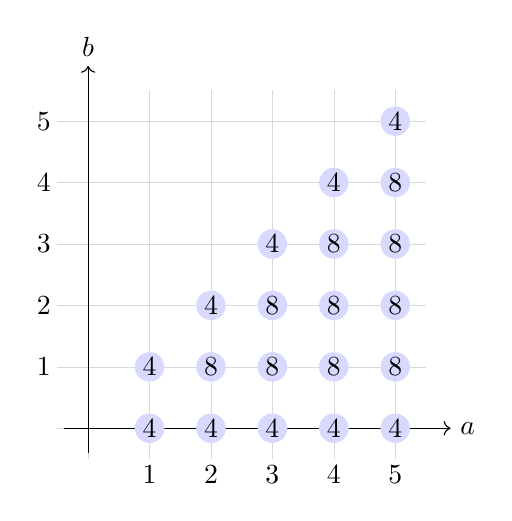
\begin{tikzpicture}[x=0.78cm,y=0.78cm]
\draw[step=1,gray!30,very thin] (-0.5,-0.5) grid (5.5,5.5);
\draw[->] (-0.4,0)--(5.9,0) node[right] {$a$};
\draw[->] (0,-0.4)--(0,5.9) node[above] {$b$};
\foreach \a in {1,...,5}{\foreach \b in {0,...,\a}{
 \ifnum\b=0\def\n{4}\else\ifnum\a=\b\def\n{4}\else\def\n{8}\fi\fi
 \fill[blue!15] (\a,\b) circle (0.24);
 \node at (\a,\b) {\n};}}
\foreach \k in {1,...,5}{\node[below] at (\k,-0.45){\k};\node[left] at (-0.45,\k){\k};}
\end{tikzpicture}
\caption{20 个代表 $(-a,-b)$。数字表示轨道大小，而不是搜索次数。10 个边界代表的轨道大小为四，10 个内部代表的轨道大小为八，覆盖了全部 120 个规范化首手应手。坐标绝对值五也涵盖该坐标所有更大的实际绝对值。}
\label{fig:orbits}
\end{figure}

\section{独立验证与观测到的计算}
\label{sec:compute}
\subsection{检查器信任什么}
独立检查器是由八个源码文件组成、使用标准库的 Python 程序栈。它不导入搜索实现、首个检查器、RV2 或 Rapfi。它从有限集合重建规范化坐标轴插入和五连段；重建符号规则的关键应手；检查序列的充分条件；并遍历完整的模块化证明闭包。在开局层，它重建 $R$，检查全部 20 个根节点和全部 120 个代表分配，验证每个对称矩阵，并要求从空棋盘解释结果。
断言必须保持启用；使用 Python 的 \code{-O} 选项执行会被拒绝。保存的回执是此前计算的证据，不能替代最终运行中的重新数学检查。


下表标识冻结的本地记录。摘要不能代替完整证书交付或新鲜核验。
\begin{center}\scriptsize
\begin{tabular}{@{}ll@{}}
空盘覆盖 & \texttt{fce6b466f2675cb5a76f40b1e979fb77bdfc4abc6971971510e1c60196adf85c}\\
数学核验结果 & \texttt{9720a055b970aa092dc216ca73059055d97d040ae3c47a31f357b26a7b40443b}\\
字节审计 & \texttt{226562fd83b790dbce3f076aedad58e7ff22f9ec4d8da78fe29982cd448b90f4}
\end{tabular}\end{center}

\subsection{已完成的运行与统计范围}
最终数学运行检查了全部 20 个开局根节点和全部 120 个规范化首手应手，总界为 35，且没有复用已检查文件的回执。观测到的进程以状态零退出。20个根依次使用四工作进程池，每个观测到的工作进程均成功退出。重新运行的数学入口程序报告用时 27,837.450 秒。外层包装程序报告用时 27,837.498 秒；后者包含前者，两者不能相加。

另一次完整字节审计读取了选定的依赖闭包，并对照重新生成的回执进行检查。它报告了 1,482,906 个不同依赖路径，以及跨根节点共 1,652,612 次文件出现，用时 5,729.200 秒。不同路径不一定对应不同内容。该审计的实际进程也以状态零退出。审计期间运行了一个操作系统缓存预取辅助程序；每个摘要仍然根据实际文件字节重新计算。因此，这个时长不是冷缓存基准测试结果。

表~\ref{tab:counts} 记录了对所有开局根节点求和的出现次数。一些子证明被共享，因此这些总和与不同路径的并集大小不同。节点总数并非一局对弈中的落子数，也不是不同无限棋盘局面的数量。这些是对一个特定、已验证证明对象的观测，不是证书大小的下界。

\begin{table}[ht]
\centering
\begin{tabular}{lr}
\toprule 项目 & 观测值\\\midrule
覆盖的规范化首手应手 & 120\\
检查的对称代表根节点 & 20\\
普通证明文件出现次数 & 1,644,613\\
普通可达节点出现次数 & 109,364,098\\
包文件出现次数 & 7,999\\
包边出现次数 & 1,954,756\\
不同的选定依赖路径 & 1,482,906\\
重新数学检查的墙钟秒数 & 27,837.450\\
单独完整字节审计的墙钟秒数 & 5,729.200\\
\bottomrule
\end{tabular}
\caption{记录的证书与验证统计。出现次数可能在不同根节点之间重复。数学阶段用时、包装程序用时和审计用时，不是独立的 CPU 成本测量。不能由这些数字推断完整的从零搜索时间或整体搜索加速比。}
\label{tab:counts}
\end{table}

稿件准备时的环境为 Intel Core i7-12700H、20个逻辑处理器、Windows 11 Pro版本26200、约31.7 GiB内存及系统Python 3.13.14。这不是历史启动记录；每次复验须记录自身的实际运行时、硬件、退出状态及墙钟时间。


\subsection{规则对应与版本绑定}
附录~\ref{app:rule-use} 对每个节点标签列出数学命题、检查入口、前提及步数界。新的全量用量普查不同于数学复验；待统计表示未知，不是零。尤其不能以样例确立最终证书是否采用定理~\ref{mac:prepared} 和~\ref{mac:interruption}。

被接受的运行绑定八份检查器源码、实际根和选定证明字节。非零退出、缺失依赖、过期回执、源码或字节不匹配、覆盖不完整、规则闭包未完成，均判为失败，不能视为证明。附录~\ref{app:provenance} 记录历史失败与最终记录完整性检查。

\begin{proof}[定理~\ref{thm:main} 的证明]
已完成的独立运行接受了 20 个代表根节点证书，每个证书都具有指定规则、包含两枚实际棋子的根局面和总落子界 35，并检查了 120 个首手应手分配。
被接受的短规则和长规则具有第~\ref{sec:short} 节和第~\ref{sec:long} 节所证明的统一策略性质。由定理~\ref{thm:sound}，每个代表证书都从每个实际原像出发，在其剩余实际步数计数内获胜。随后，命题~\ref{prop:opening} 将这些策略转换到黑方在 $(0,0)$ 开始后，每个实际合法首手应手对应的局面。35 这一计数包括最初的两个落子。字节审计将这次计算绑定到选定的实际证明字节；其记录是有限计算的完整性见证，而不是关于远处行棋的额外数学假设。
\end{proof}


\section{将搜索视为不受信任的生成器}\label{sec:search}
生成器使用有限棋盘策略、RV2、Rapfi、自由规则威胁与几何排序提供黑着建议。精确五连规则和有限引擎窗口可能产生不适用建议；只有无限棋盘证书检查器验收策略。

搜索为持久化 AND/OR 计算：黑选一个动作，但须证明其全部抽象结果；白须覆盖全部抽象应手。备选黑着保持各自独立义务，已完成证明与已耗预算在恢复时保留。UNKNOWN、超时、候选耗尽与缺失分支，均不证明白胜或黑败；反胜只否决被试黑着。界35针对本证书确立，并非所有可能获胜策略的先验界。

\section{可复现性与评审材料}
\label{sec:repro}
证明材料是空盘覆盖证书及其完整选定依赖闭包，以及冻结的八份验证源码。日志、摘要、示例棋谱和论文均不能代替这些文件。评审包必须包含字节清单、许可证、源码身份、仅依赖标准库的入口、确定命令和预期输出、实测存储需求及成功运行记录。核验不依赖搜索引擎。审稿期私下交付即可，不要求先取得证明产物 DOI。

在包根目录执行以下单行命令；同样的字面文本保存于 \code{verify-command.txt}：
\begin{quote}\small
\verb|python -B verify-review.py --workers 4 --output-dir fresh-check|
\end{quote}
\code{fresh-check} 必须为新目录。预期结果为实际退出状态零，\code{release-acceptance.json} 的状态为 \code{VERIFIED\_RELOCATED\_EMPTY\_BOARD\_REVIEW\_RELEASE}，接受20个根、覆盖120个应手，总落子界35。随后完整字节审计须将结果绑定至包清单。必须启用断言。任何不匹配、非零退出、文件缺失或中断均为失败；进度记录或成功样例均不足以验收全证书。

英文第 1 版论文已公开；完整证书尚未作为可移植评审包交付。本轮材料冻结验证核，并在同一Windows主机的另一目录中完成局面示例复验；这不是隔离环境，也不是全量核验。全路径清单、规则用量普查、实测存储总量及无法访问原工作区的完整复验，均是交付关卡，其实际状态见随附修订报告。不以样例压缩率推算全证书体积。路径迁移要求见附录~\ref{app:provenance}。在完整包与隔离全量复验可用之前，计算证明的外部复核仍未完成。


\section{讨论}
远处行棋由完整插入集合及经检查的充分规则覆盖。远处威胁可能迫使真实防守，其耗时计入长规则步数界。不满足隔离或反威胁条件时必须显式展开。保守抽象可能扩大证明树；更细规则或替代黑着可缩小规模，但须各自证明可靠性并核验。接收前仍须完整交付证明产物并完成隔离全量复验。本文不主张35最优，也未确立更小的普遍远处行棋上界。

\appendix

\section{开局根的统计}\label{app:stats}
随附 \code{opening-run-statistics.csv} 保留20个根的全部观测数据。普通文件与节点数按每根出现次数计，拼接文件另计；每根秒数包含文件头、数学检查和绑定阶段，已包含于全局封装用时。覆盖证明见第~\ref{sec:opening} 节，不依赖这些诊断统计。

\section{验证器源码与字节身份}
\label{app:sources}
以下八个文件组成一套独立验证器，而不是整个定理的八套独立实现：
路径均在 \code{scripts/} 下，并带前缀 \code{reference\_}。
\begin{center}\small\ttfamily
\begin{tabular}{@{}ll@{}}
gap\_opening\_cover.py & gap\_bundle\_batched.py\\
gap\_bundle\_parallel.py & gap\_bundle\_verifier.py\\
gap\_verifier.py & infinite\_threat\_witness.py\\
prepared\_remote\_sequence.py & remote\_interruption\_sequence.py
\end{tabular}\end{center}
发表材料清单记录了它们的完整摘要、实际证明根，以及已完成的数学核验与字节审计记录。摘要检查是识别已核验版本所必需的，但它本身既不能认证执行观察者，也不能建立数学正确性。


\section{贡献与研究工具}
作者提供研究目标、策略指导与项目监督。研究探索、程序开发、调试和稿件准备使用了 OpenAI Codex 及语言模型辅助；未能为每次历史交互确定精确模型标识。RV2 与 Rapfi 提供不受信任的选点建议，其评分不是证明验收条件。独立检查器不导入搜索实现或两种引擎。本工作尚未经过外部同行评审，也未进行证明助手形式化。


\section{计算来源记录与路径迁移}
\label{app:provenance}
历史运行曾因工作池损坏、审计退出状态120、替换进度文件时的 Windows 错误5而失败，均未验收或计入成功用时。最终审计只增加有界替换重试，数学检查与哈希主体未变，持续错误仍判失败。完成关卡绑定成功运行、根、源码身份和字节，不是另一次数学遍历。后续监控页修改未改变冻结的八源验证核。

所有引用必须在评审包内部解析。POSIX 上的 Windows 反斜线须按字段结构处理。改写证明文件会改变它及所有绑定它的祖先摘要，因此转换包需要新的完整数学检查和字节清单；新的路径加载器也需审查。原验收字节与历史回执保持冻结。发布复验必须无法访问原工作区。原产物评估中的 39 文件压缩样本既不是完整包，也不能据此推算全体存储需求。


\section{规则用量与检查入口对应}
\label{app:rule-use}
% 与英文表同口径。完整闭包统计完成前，用量 pending 不能解释为零。
\providecommand{\RuleCount}[1]{\textit{待统计}}



\begingroup\scriptsize\setlength{\tabcolsep}{2pt}\renewcommand{\arraystretch}{1.12}
\begin{longtable}{@{}>{\raggedright\arraybackslash}p{.25\linewidth}>{\raggedright\arraybackslash}p{.07\linewidth}>{\raggedright\arraybackslash}p{.09\linewidth}>{\raggedright\arraybackslash}p{.39\linewidth}r@{}}
\caption{数学规则、程序检查与最终证书用量。用量按20个开局根累加每份普通证书中从根可达的节点，不是不同局面数或执行路径数。}\label{tab:rule-use}\\
\toprule
节点规则 & 命题 & 入口 & 检查前提；额外实际落子数 & 用量\\
\midrule
\endfirsthead
\toprule
节点规则 & 命题 & 入口 & 检查前提；额外实际落子数 & 用量\\
\midrule
\endhead
\texttt{terminal} & \ref{thm:sound} & G.v & 黑刚成五且白无五；$0$。 & \RuleCount{COUNT_terminal}\\
\texttt{black} & \ref{lem:black} & G.v & 相对黑着合法，覆盖其全部后继；每边$1$。 & \RuleCount{COUNT_black}\\
\texttt{white} & \ref{lem:white} & G.v & 覆盖全部规范化白后继；每边$1$。 & \RuleCount{COUNT_white}\\
\texttt{double\_\allowbreak immediate\_\allowbreak win} & \ref{mac:double-completion} & G.v & 白无即时获胜点；黑有至少两个；$2$。 & \RuleCount{COUNT_double_immediate_win}\\
\texttt{double\_\allowbreak open\_\allowbreak four} & \ref{mac:double-completion} & G.v & 与双完成规则相同前提；$2$。 & \RuleCount{COUNT_double_open_four}\\
\texttt{next\_\allowbreak turn\_\allowbreak finish} & \ref{mac:finish-critical} & G.v & 每个白后继中白无五且黑有获胜点；$2$。 & \RuleCount{COUNT_next_turn_finish}\\
\texttt{white\_\allowbreak critical} & \ref{mac:finish-critical} & G.v & 白后继均无白五；保留全部黑无获胜点的后继；省略支$2$。 & \RuleCount{COUNT_white_critical}\\
\texttt{white\_\allowbreak open\_\allowbreak four\_\allowbreak critical} & \ref{mac:small-open-four} & G.v & 精确$(|B|,|W|)=(3,2)$；保留全部无模板后继；省略支$4$。 & \RuleCount{COUNT_white_open_four_critical}\\
\texttt{white\_\allowbreak forced\_\allowbreak block\_\allowbreak symbolic} & \ref{mac:forced-block} & G.c & 白无获胜点且黑有；保留其防点；省略支$2$。 & \RuleCount{COUNT_white_forced_block_symbolic}\\
\texttt{white\_\allowbreak fork\_\allowbreak symbolic} & \ref{mac:fork} & G.c & 刚性双杀，完整防点及白反冲四；省略支$4$。 & \RuleCount{COUNT_white_fork_symbolic}\\
\texttt{white\_\allowbreak open\_\allowbreak four\_\allowbreak symbolic} & \ref{mac:template-family} & G.c & 选取同一刚性框架中的模板族并保留反冲四；省略支$4$。 & \RuleCount{COUNT_white_open_four_symbolic}\\
\texttt{white\_\allowbreak open\_\allowbreak four\_\allowbreak symbolic\_\allowbreak shared} & \ref{mac:template-family} & G.c & 至少五黑；模板共享旧黑支持点；省略支$4$。 & \RuleCount{COUNT_white_open_four_symbolic_shared}\\
\texttt{white\_\allowbreak open\_\allowbreak four\_\allowbreak symbolic\_\allowbreak component} & \ref{mac:template-family} & G.c & 至少五黑；模板支持点属于同一旧刚性分量；省略支$4$。 & \RuleCount{COUNT_white_open_four_symbolic_component}\\
\texttt{white\_\allowbreak open\_\allowbreak four\_\allowbreak symbolic\_\allowbreak far} & \ref{mac:template-family} & G.c & 至少六黑；两个模板存在距离大于$8$的支持点；省略支$4$。 & \RuleCount{COUNT_white_open_four_symbolic_far}\\
\texttt{infinite\_\allowbreak threat\_\allowbreak sequence} & \ref{mac:infinite} & I.v & 全部黑子在$C$；局部闭包；远白无三；包络分离及$M$；$L\le H-p$。 & \RuleCount{COUNT_infinite_threat_sequence}\\
\texttt{prepared\_\allowbreak remote\_\allowbreak threat\_\allowbreak sequence} & \ref{mac:prepared} & P.v & 局部闭包；远三已堵；远棋包络避$E$；$M$；$L\le H-p$。 & \RuleCount{COUNT_prepared_remote_threat_sequence}\\
\texttt{remote\_\allowbreak interruption\_\allowbreak threat\_\allowbreak sequence} & \ref{mac:interruption} & R.v & 完整局部及远程闭包；唯一防点；包络分离；全部记录态$MI$；$L+2\sum_jN_j\le H-p$。 & \RuleCount{COUNT_remote_interruption_threat_sequence}\\
\bottomrule
\end{longtable}
\endgroup
\begingroup\par\smallskip\footnotesize\raggedright
G、I、P、R依次表示\texttt{scripts/}下的\texttt{reference\_gap\_verifier.py}、
\texttt{reference\_infinite\_threat\_witness.py}、
\texttt{reference\_prepared\_remote\_sequence.py}和
\texttt{reference\_remote\_interruption\_sequence.py}；v表示\texttt{verify}，c表示\texttt{critical\_actions}。
除终局外，均检查非终局、正确轮次和实际步数；保留着法必须覆盖其全部规范化后继。
模板规则均保留完整白反冲四集合。分文件黑白节点由
\texttt{reference\_gap\_bundle\_verifier.}\allowbreak\texttt{verify\_file}检查同样的显式规则，用量另计。


\par\endgroup

\section{完整的双远处分量实例}\label{app:remote-example}
示例证书 \code{two-remote-components-example.json} 的已规范化根如下，共已有18次实际落子，轮到黑棋。此例用于说明规则，不增加开局覆盖。
\begin{center}\small
\begin{tabular}{@{}lll@{}}\toprule
框架 & 旧黑子 & 旧白子\\\midrule
$C$ & $(0,0),(1,-1),(1,0),(3,4),(4,3)$ & $(1,3),(2,3),(3,3)$\\
$Q_1$ & $(-8,1),(-8,2)$ & $(-7,0),(-6,-1),(-5,-2)$\\
$Q_2$ & $(8,10),(8,11)$ & $(9,9),(10,8),(11,7)$\\\bottomrule
\end{tabular}\end{center}
局部增子依次为 $(1,-2),(2,-2),(0,-2),(2,0),(-1,0)$，前四个为活三，最后一个为活四。对应防点集依次为 $\{(1,-3),(1,1)\}$、$\{(3,-3),(-1,1)\}$、$\{(-1,-2),(3,-2)\}$、$\{(-1,-3),(3,1)\}$、$\{(-2,0),(3,0)\}$。完整局部闭包的界为 $L=13$，活动集有33点，28个记录态包括初态、增子后态、封点后态及加入虚拟防点后态。未记录的局部白冲四中间态由引理~\ref{mac:intermediate} 处理。

局部反冲四可在 $(0,3),(-1,3)$ 中任选一点，黑封另一点。两个远处图对应的点对分别为 $(-4,-3),(-3,-4)$ 和 $(12,6),(13,5)$。每图记录初态、两个白冲四中间态、两个黑封点后态；封点后均无后续边，所以 $N_1=N_2=1$。两核完整重建图、包络与混合线条件，得到后续界 $13+2(1+1)=17$，总界35。随附记录态文件给出完整状态集合。

\paragraph{策略执行。}
依次走规定局部增子，成五立即结束。在每个白棋决策点，按以下顺序处理实际应手：
\begin{enumerate}\setlength{\itemsep}{0pt}\setlength{\parsep}{0pt}
\item 当前为冲四或活四且黑仍有完成点时，直接成五并结束。
\item 应手属于 $K$：将全部 $K$ 加入虚拟 $D$，计一次局部实际落子，前进至下个增子。
\item 否则，三子算子的应手若产生白完成点，按其纯框架支持走局部闭包或对应远处图，黑封唯一完成点并留在当前算子。分别计两次局部落子或两次远处落子；黑封点若成五则结束。
\item 否则转入该算子的快速终结，结束且不返回模拟。
\end{enumerate}
被检查的条件排除每个决策点上的白方获胜。局部计数至多 $L$；任何交错次序的远处计数至多 $2\sum_jN_j$。例如首增子后，白在 $(1000,1000)$ 安静落子，黑可在 $(1,1)$ 扩展，再在 $(1,-3)$ 或 $(1,2)$ 完成。

随附记录态文件还列出一条合法续谱，包含两次远处中断、一次局部反冲四及通常防守，最终在总第35手黑胜。该路径说明完整证书，不能代替全部分支检查。

\begin{thebibliography}{99}
\setlength{\itemsep}{0pt}\setlength{\parskip}{0pt}
\bibitem{Allis1993} L. V. Allis, H. J. van den Herik, and M. P. H. Huntjens.
Go-Moku solved by new search techniques. AAAI Fall Symposium on Games:
Planning and Learning, 1993.
\bibitem{Allis1996} L. V. Allis, H. J. van den Herik, and M. P. H. Huntjens.
Go-Moku solved by new search techniques. Computational Intelligence
12(1) (1996), 7--23.
\url{https://doi.org/10.1111/j.1467-8640.1996.tb00250.x}.
\bibitem{Erde2012} J. Erde. An $n$-in-a-row game.
arXiv:1209.5123v1, 2012.
\url{https://arxiv.org/abs/1209.5123}.
\bibitem{Hefetz2014} D. Hefetz, M. Krivelevich, M. Stojakovi\'c, and T. Szab\'o.
Positional Games. Oberwolfach Seminars 44, Birkh\"auser, 2014.
\url{https://doi.org/10.1007/978-3-0348-0825-5}.
\bibitem{Gyorffy2019} L. Gy\H{o}rffy, G. Makay, and A. Pluh\'ar.
The pairing strategies of the 9-in-a-row game.
Ars Mathematica Contemporanea 16(1) (2019), 97--109.
\url{https://doi.org/10.26493/1855-3974.1350.990}.
\bibitem{Pluhar2022} A. S. Pluh\'ar. One and two-person Positional games.
为取得 MTA Doktora 头衔而提交给匈牙利科学院的论文，Szeged，标题页日期为 2022 年；于 2023 年存入 REAL-d。
\url{https://real-d.mtak.hu/1545/}.
\bibitem{Hamkins2023} J. D. Hamkins and D. Leonessi.
Infinite Hex is a draw. Integers 23 (2023), G6.
\url{https://doi.org/10.5281/zenodo.10075843}.
\end{thebibliography}
\end{document}

